\chapter{Background}
This section will introduce various fundamental topics that were taken into consideration in the design of the aerial software defined radio platform developed in this MQP. The topics include but are not limited to, spectrum allocation, energy detection, wireless transmitter localization, software defined radio, and aerial flight platform.

\section{Spectrum}
\subsection{Spectrum Usage}
The spectrum of radio frequencies used for wireless communications is managed by the government to promote efficient use and net social benefit. The National Telecommunications and Information Administration (NTIA) and the Federal Communications Commission (FCC) regulates the allocation of these frequencies in the United States as shown in Figure \ref{fig:freq_chart} below (A larger diagram can be located at the Appendix).
\begin{figure}[ht]
\centering
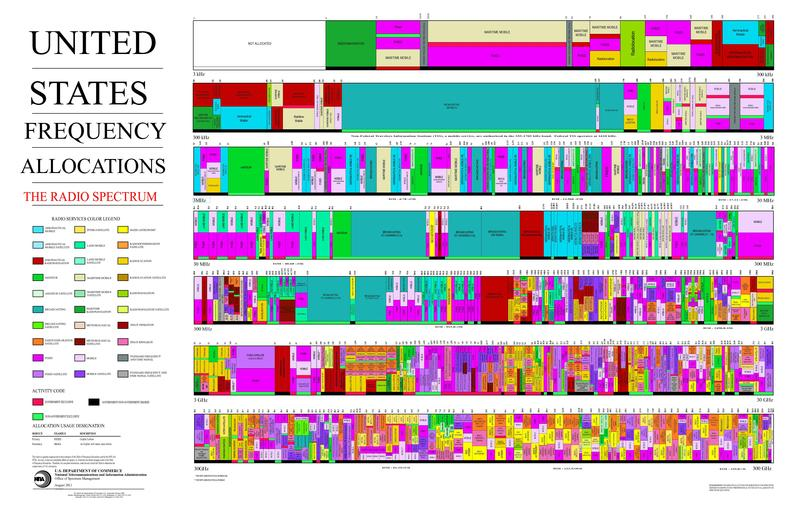
\includegraphics[width=0.70\textwidth]{img/the_radio_spectrum.jpg}
\caption{United States Frequency Allocation Chart}
\label{fig:freq_chart}
\end{figure}
As seen from the figure above, the spectrum is divided into smaller chunks where only specified entities can utilize legally. The usage of each chunk is determined by whether the NTIA and FCC require a license to use the band or not. Only operators with a license from the government can operate in the licensed bands, with uses that include AM broadcasting, FM broadcasting, and cellular communication. However, unlicensed bands are open to any entity that wants to utilize them, but they must still follow certain guidelines for usage. Technologies that use unlicensed bands include microwave, bluetooth, and WiFi.

\subsection{Cellular}
The initial goal of this MQP was to look at transmissions in the cellular band in the United States. This band, regulated by the FCC, ranges from 824MHz - 896MHz and 1850MHz - 1990MHz. The United States is divided into 734 geographic markets called Cellular Market Areas (CMAs). To operate at a certain frequency in a CMA, mobile operators must place bids on each area individually. These frequencies all use various modes for communication including Analog, Digital, TDMA, CDMA, and GSM. However, the most popular mode now is LTE telecommunications.

\subsection{Wi-Fi}
Wi-Fi first came about in 1985, when the FCC decided to open up several bands of wireless spectrum for use without a government license. In the early 1990s, the Institute of Electrical and Electronics Engineers (IEEE) realized that wireless communications needed to be standardized. A committee was formed that focused on providing a reliable, fast and robust wireless solution that would be able to scale for years to come. Thus the 802.11 standard was created in order to assure these things. Since then, there has been multiple iterations of the standard, and five sub-standards have been established for wireless communications called:802.11a, 802.11b, 802.11g, 802.11n, and 802.11ac. The spectral signature of these protocols depend on the protocol that is used. Wifi traffic can be transmitted using a bandwidth of 20 MHz, 40 MHz or 80 MHz on either the 2.4GHz band or the 5GHz band. This is dependant upon the protocols shown in Figure \ref{fig:wifi_table} below:
% table
\begin{figure}[ht]
\centering
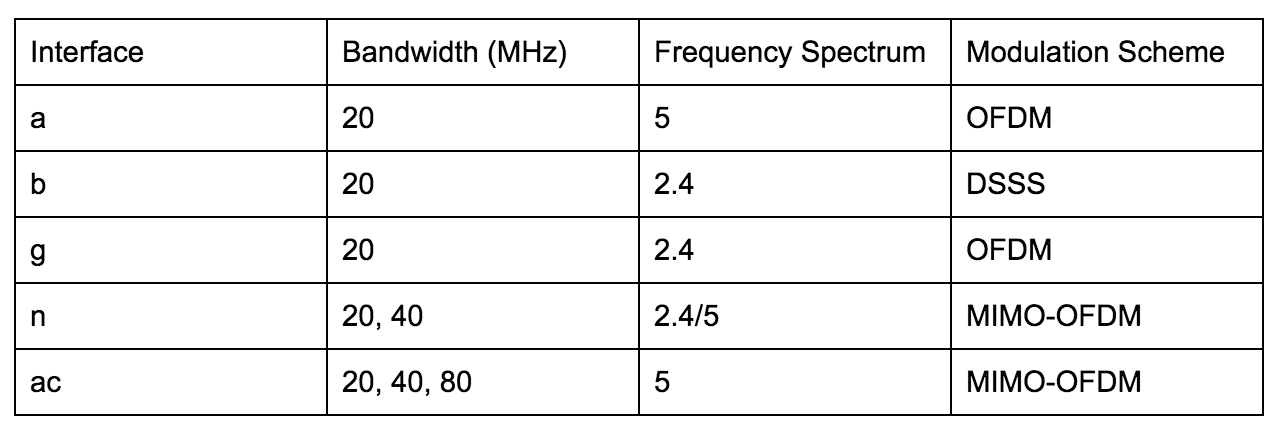
\includegraphics[width=0.70\textwidth]{img/wifi_table.png}
\caption{Wifi Table}
\label{fig:wifi_table}
\end{figure}\par
These transmissions can vary when it comes to the entire frames information. However, each standard has a preamble that signifies the start of a transmission, shown in Figure \ref{fig:wifi_preamble}.
\begin{figure}[ht]
\centering
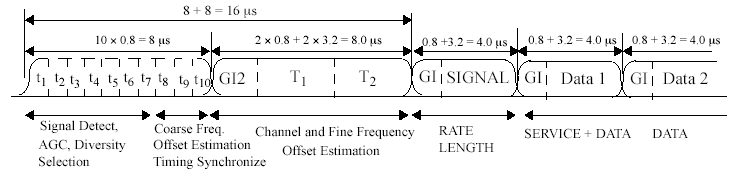
\includegraphics[width=0.70\textwidth]{img/ofdm_preamble.jpg}
\caption{Wifi Transmission Packet Preamble}
\label{fig:wifi_preamble}
\end{figure}\par
The preamble is useful to detect the start of a wifi transmission. In addition to the preamble, you could also decode the information from the Data fields, however, all of that data is usually encrypted so that it prevents any unauthorized user from accessing it. \cite{wifi_book}

\subsubsection{MAVLink}
MAVLink is a wireless communication protocol similar to wifi that is used on small unmanned aerial vehicles. The protocol was designed to be a lightweight, header-only message marshaling library, and is used by many drones as a communication protocol between the drone and the controller. MAVlink utilizes the 2.4 GHz band along with WiFi, therefore the only way to differentiate between the two signals is by comparing the frames of the two protocols. This can be done by demodulating the GFSK signal and decoding the frame which is shown in Figure \ref{fig:MAVlink_frame}. The red STX frame signifies the start of a transmission. This frame will always be an 8 bit code of 0xFE. The rest of the frame is described in Table \ref{fig:MAVlink_frame_table}.
\begin{figure}[ht]
\centering
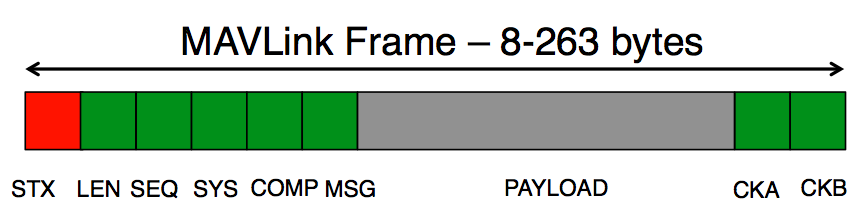
\includegraphics[width=0.70\textwidth]{img/mavlink-packet.png}
\caption{MAVLink Transmission Frame}
\label{fig:MAVlink_frame}
\end{figure}
\begin{figure}[ht]
\centering
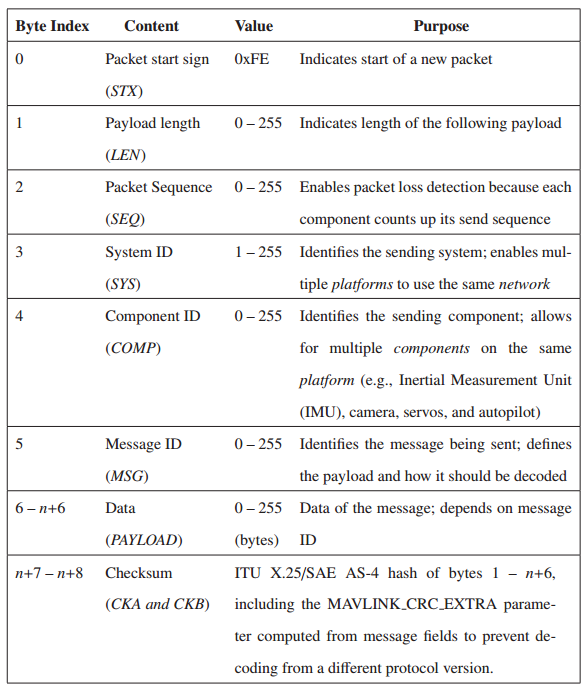
\includegraphics[width=0.70\textwidth]{img/MAVLink-Packet-Table.png}
\caption{MAVLink Frame Descriptor}
\label{fig:MAVlink_frame_table}
\end{figure}
\cite{mavlink_vuln}\par
Also, opposed to wifi signals, MAVLink transmissions are all non-encrypted which such as network attacks or an unauthorized user operating the drone. Any user can send signals to a drone using a GFSK transmitter and the drone has no knowledge on who the correct user.

\subsection{GPS}
Global Positioning System, or GPS, provides highly accurate location information to a user with a receiver module. This technology was developed during the height of the cold war in the 1960s. (Yunck, Thomas P., Liu Chao-Han, and Randolph Ware. "A history of GPS sounding." Terrestrial Atmospheric and Oceanic Sciences 11.1 (2000): 1-20. ) GPS works by using a network of 24 satellites that are transmitting on 1575.42Mhz using a division coding scheme. The individual satellites send out information such as the current system time, and their locations. Given the locations of the satellites, as well as the calculated time of travel from the satellites to the receiver, the GPS receiver then performs localization based on this received information. The accurate time stamping required to perform this localization is only possible because each GPS satellite is capable of maintaining a highly accurate clock, and each receiver determines its current time through the interpretation of satellite data. This accurate clock information is used for the synchronization of clocks across cellular telephone systems, and other time critical applications.

\section{Sensing}
As described in the previous section, the electromagnetic radio spectrum is becoming increasingly crowded, with this issue only accelerating as the Internet of Things becomes more widespread. With the conventional approach of spectrum management, users are assigned a specific frequency band. This method becomes less sustainable with increasing number of users, especially in the unlicensed frequency bands. In order to combat this, the field of Cognitive Radio (or CR) was created to utilize spectrum more efficiently. Cognitive radios are designed to provide a highly reliable connection for all users of the network, by sensing what frequencies are being used at any given moment, and utilizing the unused parts of the spectrum. The types of signals to be sensed are divided into two different groups: uncooperative users and cooperative users. The different sensing methods will be discussed in a later section. \par
The process of spectrum sensing is made more complicated by uncertainties in the received data, including channel uncertainty and noise uncertainty. With channel uncertainty, the received signal strength can fluctuate based on characteristics of the channel, such as channel fading or shadowing. Noise uncertainty refers to the fact that the power of the noise is unknown to the receiver, making it difficult to achieve a specific sensitivity. In order to have a functioning CR, both uncertainties need to be addressed. \par
As the types of signals to be sensed are split into non-cooperative and cooperative systems, so too are the methods of sensing. As the present MQP involves passive sensing of the spectrum, only the methods concerning the former will be discussed.

\subsection{Energy Detection}
The most fundamental method of non-cooperative sensing is energy detection. In this approach, the power spectral density (or PSD) of the received signal is taken. The power spectral density represents the measure of a signal’s intensity in the frequency domain computed through the fast fourier transform of a signal. This is then bandpass filtered to contain only the frequency bands being watched. These frequency bands are then integrated, to determine how much energy is present in the band. If this passes a certain threshold, the frequency band is marked as occupied.
\begin{figure}[ht]
\centering
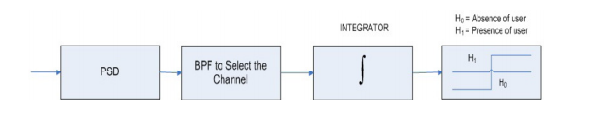
\includegraphics[width=0.70\textwidth]{img/energy_detection.png}
\caption{Energy Detection}
\label{fig:energy_detection}
\end{figure}\par
This method of detection is the most fundamentally simple, as it does not require information about the signal ignoring key aspects of signals such as modulation method and pulse shaping. Because of this, it is the simplest detection method to implement. However, the fundamental assumption made in using energy detection is that the signals being searched for have significantly more power than the noise and interference of the channel. This does not always prove to be true. In addition to this, energy detection cannot be used to distinguish signals using the frequencies measured, as no pulse shape information is determined.

\subsection{Match Filter}
Another approach to spectrum sensing is through the use of match filters. Match filters are designed to maximize the signal to noise ratio given an input signal. To operate signal sensing through match filtering, prior knowledge of the reference signal to be detected must be known. The reference signal will be correlated with the incoming signal, which means that the two signals are overlapped to determine whether any distinct similarities exist between those signals.
\begin{figure}[ht]
\centering
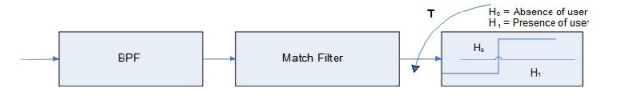
\includegraphics[width=0.70\textwidth]{img/match_filter.png}
\caption{Match Filter}
\label{fig:match_filter}
\end{figure}\par
Match filters fundamentally relies on prior knowledge of the characteristics of signals to be detected, otherwise this method will not perform with accuracy. The prior knowledge constraint limits the use of signal detection when unexpected signals are involved. Furthermore, match filter detection is optimal with stationary gaussian noise to hinder distortion. This will limit the real world applications for signal detection with match filtering as a significant portion of signal emitting devices are mobile.

\subsection{Cyclostationary Feature Detection}
Cyclostationary Feature Detection (or CFD) depends on the fact that all communication schemes have some sort of signal repetition as a core aspect. A signal with this kind of repetition is called a Cyclostationary Process\cite{cyclostat_journal}. Because of this property, when you correlate the signal with itself (or autocorrelation), there will be repeated peaks. The periodic nature of the signal also means that the autocorrelation will be periodic as well. This allows it to be expressed as a Fourier Series, called the Cyclic Autocorrelation Function (CAF) and denoted by $R_x^\alpha(\tau)$.\par 
\[R_x^\alpha(\tau)=lim(t->\infty) \frac{1}{T} \int_-T/2^T/2 R_x(t,\tau)exp(-j2\pi\alpha t dt\]
Where $R_x(t,\tau)$ is just the autocorrelation function of x at t with x at $\tau$. This function gives us an understanding of the times when the signal repeats, but is missing vital information of the repeated frequencies. By taking the fourier transform of $R_x^\alpha(\tau)$, we can get a better understanding of the frequencies in the Cyclostationary Process. This is denoted as $S_x^\alpha(f)$, and equals: \par
\[ S_x^\alpha(f)=\int_-\infty^\infty R_x^\alpha(\tau)exp(-j2\pi f\tau d\tau \]
This is called the Spectral Correlation Function (SCF). When it is normalized, it becomes the Spectral Coherence Function (SOF):
\[C_x^\alpha(f) = \frac{ S_x^\alpha(f)}{ (S_x^\alpha(f+\alpha/2) S_x^\alpha(f-\alpha/2))^{1/2}} \]
The SOF is from between 0 and 1, and represents the strength of the periodicity at that point. By plotting this value, the unique response of the Cyclostationary Process can be found, allowing for it to be categorized. \par
One of the major benefits of CFD is that it is not nearly as affected by noise. Under the generally held assumption that noise is white and Gaussian, there is no periodic response, and as such noise is not factored into CFD. A block diagram of an implementation of CFD is shown in Figure \ref{fig:cyclo_detection} below. \par

The primary downside to Cyclostationary Feature Detection is the complexity and time required to properly utilize it. The complexity lies in the number of integrals and correlations that need to be computed in order to implement CFD. In addition, the system needs to listen for signal long enough for the Cyclostationary Process to repeat. Because of these downsides, it is not common to be used on embedded systems. \par


\section{Localization}
Once a signal has been identified on a measured frequency, the next step is localization. Localization refers to the act of determining the location of a transmitted signal \cite{local_conf}. There are many different methods for localization. However, a lot of them become impractical for mobile passive sensing. In the following section, a variety of localization techniques will be discussed, as well as the practicality of implementing each of them.\par
For each of the techniques discussed below, the same basic concept is used. Three different receivers are placed around the transmitter being located. They will be called stationary nodes and the unknown node, respectively. Each stationary node gets information about its location relative to the unknown node simultaneously. For Time Difference of Arrival (TDoA), Time of Arrival (ToA), and Received Signal Strength (RSS) Localization, each stationary node calculates the distance to the unknown node. This information is used with the known locations of the stationary nodes to localize the unknown node.
Angle of Arrival (AoA) functions differently and will be described in a separate section.
\begin{figure}[ht]
\centering
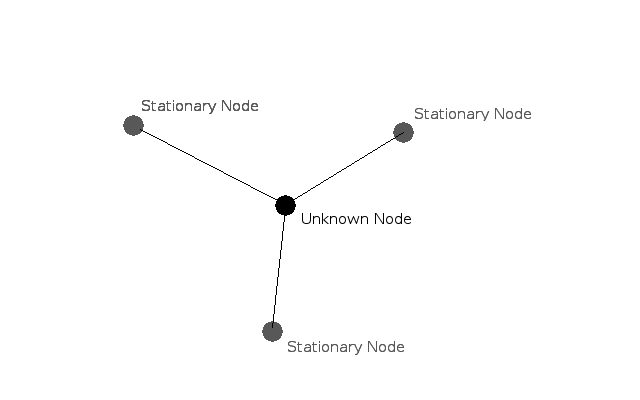
\includegraphics[width=0.70\textwidth]{img/node-localization-lines.png}
\caption{Node Localization}
\label{fig:node_localization}
\end{figure}\par
In the distance-based localization techniques, each stationary node knows the unknown node is a certain distance away \cite{local_conf}, allowing for it to be anywhere along a circle, with the stationary node in the center. By finding out where all three circles intersect, the unknown node can be located. The distance of the unknown node from any of the stationary nodes is calculated using the following equation:
\[D_i =\sqrt{(X - x_i)^2 + (Y-y_i)^2}\]\par
By plugging in the locations and calculated distance for each stationary node, a system of equations is created, making it possible to solve for the location of the unknown node.

\subsection{Time Distance of Arrival}
One method of localization is Timed Difference of Arrival (TDoA). In this method, the unknown node a signal over radio frequencies. Using the difference in the timestamp and actual time of receiving the signal, the stationary nodes can calculate the distance between each stationary node and the unknown node, using the equation \( d = c*(t_{actual} - t_{expected}) \), where c is the speed of light.
\begin{figure}[ht]
\centering
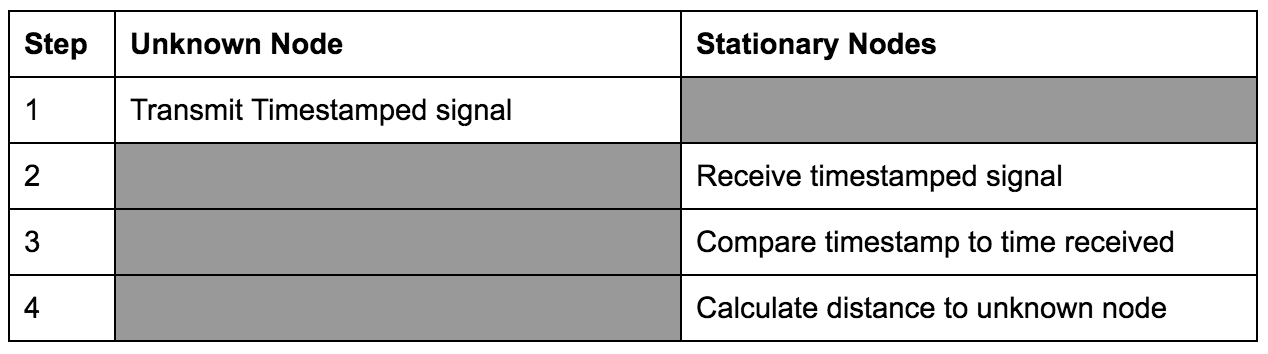
\includegraphics[width=0.70\textwidth]{img/tdoa_node_table.png}
\caption{TDoA Node Identification}
\label{fig:tdoa_node_identification}
\end{figure}\par
This method of localization is dependent on three things: the synchronization of the nodes involved, the participation of the unknown node, and the existence of three or more stationary nodes. In the use case presented by this MQP, the most difficult part about this implementation is the participation of the unknown node. Since the aerial platform has no communication with the object being localized, this method is impractical.

\subsection{Time of Arrival}
Using the Time of Arrival (or ToA) approach is similar to TDoA in concept\cite{local_conf}. Each of the stationary nodes sends a signal at a specific time, known to the unknown node. Using the difference in the known time and the time that the base receives the signal, the unknown node calculates the time the signal was in the air, and uses the speed of an electromagnetic wave to determine the distance to the stationary node, as described above. With three of these, the location of the unknown node can be triangulated.
\begin{figure}[ht]
\centering
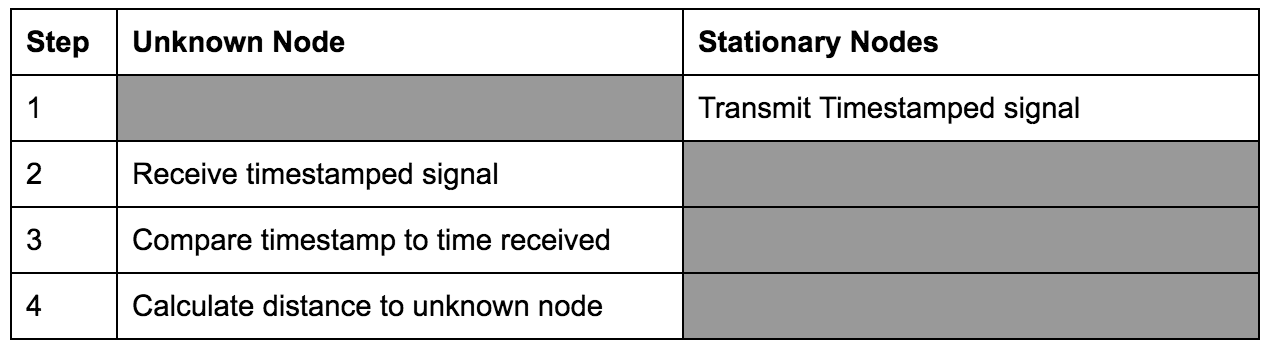
\includegraphics[width=0.70\textwidth]{img/toa_node_table.png}
\caption{ToA Node Identification}
\label{fig:toa_node_identification}
\end{figure}\par
Like TDoA, ToA requires the synchronization of the nodes involved. In most implementations, this is done using digital timestamps. It also requires the participation of the unknown node. SImilarly to TDoA, these requirements make ToA an impractical fit for this MQP.

\subsection{Received Signal Strength Localization}
Unlike the previous two methods, which depend on knowing the time a signal was sent, received signal strength localization uses the strength of a received signal to localize the unknown node\cite{local_conf}. Each of the stationary nodes receives the signal being output by the unknown node. Using the equation shown below\cite{rss_calc}, the stationary nodes can calculate the distance to the unknown node.
\[Pr = \frac{P_t G_t G_r}{4πr^2} \]\par
Because RSSI localization depends on the measurement of the signal strength, it is adversely affected by sources of noise and interference, like channel fading and multipath interference\cite{local_conf}. This makes the technique have lower accuracy. The effects of noise and shifting channels can be somewhat mitigated by averaging the RSS data.

\subsection{Angle of Arrival}
Unlike the previously described methods, ome localization techniques use the angle that the signal arrives at relative to a reference direction, or the Angle of Arrival (AoA)\cite{local_aoa}. To use this method, antenna arrays or directional antennas are used to determine the angle at which the signal arrived at. Similarly to TDoA, the stationary nodes wait for a signal from the unknown node. Using the directional antenna or the antenna array, the AoA is calculated at each stationary node. From each of these nodes, a ray can be drawn originating from the node that follows the angle of arrival. The unknown node is located based on where the rays intersect.
\begin{figure}[ht]
\centering
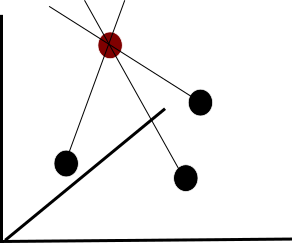
\includegraphics[width=0.70\textwidth]{img/path4188.png}
\caption{Angle of Arrival Diagram}
\label{fig:aoa_diagram}
\end{figure}\par
AoA localization consists of similar issues as other techniques. Noise and channel issues still come into effect. Additional issues occur if these unknowns can’t be dealt with. Another constraint is the requirement for highly directional sensing, which complicates the sensing of a signal before localizing it.

\section{Software Defined Radio}
Due to the rapidly increasing number of users dependent on efficient spectrum allocation for communication, the use of reprogrammable radios has become an integral part of designing communication systems. Radios exist in a wide range of devices, such as cell phones, cars, televisions, garage door openers, and computers.A radio is any device that transmits or receives wireless signals that are within the radio frequency band of the electromagnetic spectrum. A software defined radio (SDR) is defined as a “radio in which some or all of the physical layer functions are software defined”.\cite{sdr_forum} \par
Traditional hardware based radios are nearly impossible to modify post-production, and have limited ways to be repurposed. The Wireless Innovation Forum states that this results in higher production costs and minimal capabilities in supporting multiple waveform standards.\cite{wireless_innovation} SDRs, on the other hand, are comparatively inexpensive, highly reusable, and are easily configurable to support multiple waveform standards. They can be implemented on field programmable gate arrays (FPGA), digital signal processors (DSP), programmed System on Chips (SoC), general purpose processors (GPP), personal computers (PC), or other reprogrammable application specific integrated circuits (ASICs). The use of these reprogrammable technologies allows for the possibility of constant updates or dynamic radio systems without the need to add additional hardware. \par
The primary goal of designing a software defined radio is to implement as much of the radio in the digital space, minimizing the use of analog components. The digital portion of an SDR performs the data compression, encoding, modulation, demodulation, decoding, and decompression in software. The only analog components are a digital to analog converter (DAC), an analog to digital converter (ADC), and a simple RF circuit. The DAC and ADC serve as the bridge between the analog and digital realms enabling the software defined signal to be converted to an analog one to transmit and receive, then converted back to digital on the receiving end shown below in Figure \ref{fig:sdr_flow_diagram}
\begin{figure}[ht]
\centering
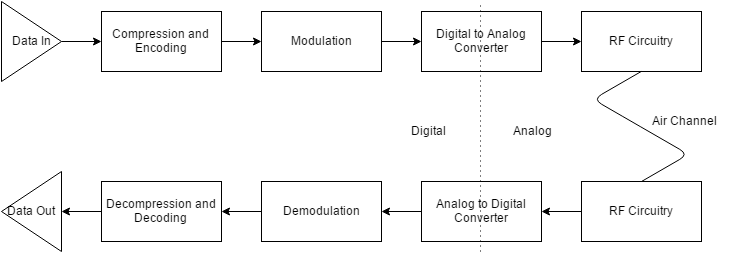
\includegraphics[width=0.70\textwidth]{img/sdr_diagram.png}
\caption{Flow diagram of an SDR with the distinction between the digital and analog components}
\label{fig:sdr_flow_diagram}
\end{figure}\par
A software defined radio has the capability to be much more sophisticated than an analog counterpart, such as an adaptive radio. Adaptive radios are able to monitor their own performance and adjust their parameters to ensure the highest quality of service.\cite{cog_radios} A more advanced type of adaptive radio is the cognitive radio, mentioned in section 2.2.3, which is able to monitor, sense, and detect conditions of their operating environment and adjust its characteristics to match those conditions. This allows the radio to provide improved performance and quality of service. These radios are able to find and transmit on open gaps in a radio spectrum. This allows for minimal interference from other sources. Cognitive radios use the trends of the channel to determine whether to switch channels or continue using the current channel. The most advanced type of adaptive radio is the intelligent radio. These radios are capable of machine learning which enables the radio to improve its algorithms for adjusting the radio's parameters based on previous experience when changes to performance or the environment occur.\cite{int_radio} The relationship between these types of radios is shown below in Figure \ref{fig:sdr_relationship_diagram}
\begin{figure}[ht]
\centering
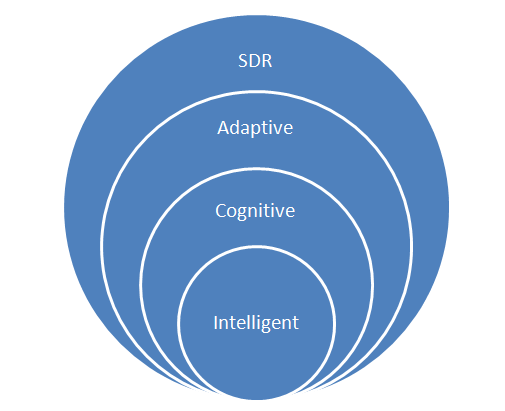
\includegraphics[width=0.70\textwidth]{img/sdr_diagram2.png}
\caption{The relationship between SDR, adaptive radio, cognitive radio, and intelligent radio}
\label{fig:sdr_relationship_diagram}
\end{figure}\par
A typical transmitter will pass a modulated signal to the DAC which will take the digital input and output a baseband analog signal. The analog signal will be upconverted to the carrier frequency in a single step or multiple steps. The receiver will take the received analog signal and downconvert it. It then passes the baseband analog signal to the ADC to convert the signal back into digital for the SDR to process. The capabilities of the ADC and DAC, such as the as the bandwidth and noise tolerance of these two components, will dictate the complexity the RF circuitry that is needed to satisfy these requirements.\par
While it is currently not possible to directly transmit from the ADC, future technological advances may make this possible. An ADC and DAC having the ability to convert the signal without the need for up or downconversion would allow for the direct connection of the ADC or DAC to the antenna. This would allow for wide band reception capability and tolerance to varying input power levels.\cite{soprano_sdr}

\section{Aerial Platforms}
The inspiration behind this MQP was to discover how much information could be gleaned from the wireless spectrum when observed from the air. To facilitate this, three main mobile methods of elevating the sensory unit were considered: kites, fixed-wing aircraft, and multicopters, each of which will be described in detail below.

\subsection{Kites}
A kite is a passive structure tethered to the ground that stays airborne by catching wind. There are many different styles of kite, including parafoil, rokkaku, delta, and sled, but they all rely on the same principle to fly.\cite{kite_iqp} Kites have near unlimited flight time and high payload capacity when operated in favorable conditions, but in exchange they sacrifice control, reliability, and maneuverability.\par
Since kites are powered by the natural wind in the atmosphere, they do not require any power to stay aloft. Depending on the style of kite however, they do require specific conditions to fly. Almost all kites need at least 2-3 mph of wind to get up into the air, and delta and rokkaku are limited to a maximum of 12-16 mph.\cite{kite_iqp} Parafoils can fly in wind up to 20 mph, but can be unstable\cite{kite_iqp}.\par
The only control a user has over a kite in flight is changing its height by letting out or reeling in more of the tether cord. Different styles of kite have different flying angles, which impacts the amount of weight they can carry. Some kites, such as the rokkaku and delta styles, can be modified during assembly to change their angle of flight, where higher angles produce more lift. While parafoils can inherently carry more weight, they also have a low flying angle, which can be problematic in some scenarios. The preparation for flight involves assembling the kite, normally by inserting cross-bars, and unreeling the tether in an open space that allows the kite to take off.\par
Kites are, by necessity, constructed of very light materials and cannot support much extra weight in light wind situations. Again, the style of kite affects the carrying capacity: deltas can carry a moderate amount of weight, but need higher winds to stay aloft. Parafoil and rokkaku kites can carry more weight, with 10 lbs being on the low end. All things considered, kites have great flight time and payload capacity, but they are susceptible to poor weather and have little to no maneuverability or user control over movement.

\subsection{Fixed-wing Aircraft}
A fixed-wing aircraft is a rigid structure with one or more rotors oriented forward that gains lift from the flow of air over its wings. An aircraft’s movement is controlled by servos onboard that move flaps to change the surface of the aircraft, in turn changing the dynamics of flight and causing the plane to respond. They are very efficient in terms of the ratio of flight time to power used because the lift comes from the shape of the wings, not the speed of the motor. Since the lift comes from the wings, fixed-wing aircraft have a moderate flying time and can carry a moderate amount of weight, but the plane’s motion is very linear so its maneuverability is limited.\par
The flight time of most battery powered remote-control fixed-wing aircraft is around half an hour assuming some aerobatics. In a surveying role, with the plane flying low circles, the flight time would likely increase slightly. There are also gasoline powered aircraft with small engines onboard to power the main propeller. Gasoline has a very high energy density, so it’s possible to fly for multiple hours with a gasoline powered aircraft.\par
Fixed-wing aircraft have a fairly lenient payload capacity. One thing to consider about adding payloads to fixed-wing aircraft is that since the aircraft’s flight is so heavily impacted by the body shape, any payload will need to be incorporated into the body of the aircraft to minimize airflow disturbance. To get more lift, and thus carry more weight, the plane simply needs to fly faster to force more air over the wings. This has drawbacks however, as spinning the propeller faster will drain the power source faster and decrease maneuverability.\par
A fixed-wing aircraft is able to cover large distances flying laterally, but it is not able to stop mid-flight and hover in place. Its turning radius is often quite large, and it must not drop below a certain speed to remain airborne. While fixed-wing aircraft are mobile, they are not very agile. Most fixed-wing aircraft require a long flat runway to takeoff and land on, limiting the number of locations in which they could reasonably launch. In addition, fixed-wing aircraft are much larger and are commonly disassembled for transport. All things considered, fixed-wing aircraft have a lot of conditions that inhibit their usefulness even though they have fairly good flight time and payload capacity.

\subsection{Multicopters}
A multicopter, sometimes also called a drone, is a flying device with two or more upward oriented rotors. A typical multicopter structure will have an even number of fixed-pitch propellers (often 4, 6, or 8), powered by electric motors placed equidistant from the center of mass. To have full control over the movement of the quadcopter, at least 3 rotors are needed. By controlling the speed at which the rotors spin, the multicopter can be controlled and flown. The least mechanically complex of the three devices investigated here, multicopters rely solely on software control of the rotors for lift and control. The principles behind multicopter flight lead them to be highly maneuverable, but at the cost of flight time and payload capacity.
\begin{figure}[ht]
\centering
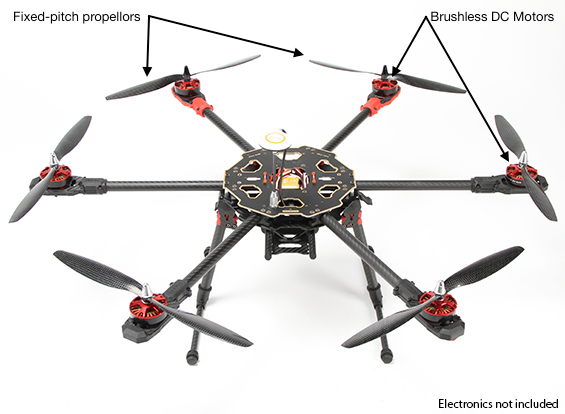
\includegraphics[width=0.70\textwidth]{img/hexacopter.jpg}
\caption{A multicopter with 6 rotors}
\label{fig:multicopter_hex}
\end{figure}\par
The primary concern when using a multicopter is the flight time. Most commercial multirotors quote flight times in the 10-20 minute range with the best performing drones topping out around 30 minutes (cite). This is because the power required to spin the electric motors fast enough to get lift can be immense, drawing up to 60 amps on takeoff. Ascending from a stationary position draws much more energy than hovering or lateral flying, so multiple takeoffs and landings in one flight will hamper the battery even more. The high current draw of the electric motors necessitates the use of Lithium Polymer (LiPo) batteries that can discharge large amounts of power very quickly. LiPo batteries have another benefit for use in multicopters and that is their low weight.\par
Weight is a very important factor in the operation of a multicopter because the amount of weight to be lifted directly corresponds to the speed the motors must be driven at to achieve lift. Multicopters in general have low payload capacities because any extra weight equates to more power that must be provided by the rotors. In effect, the more weight the drone is carrying, the less flight time it will have. This correlation forces a choice to be made over whether to prioritize flight time or amount of payload supported.\par
The most advantageous aspect of multicopters is their maneuverability. The nature of their control means it is possible to stop and start, hover in place, rotate in place, and quickly change directions and altitudes. In particular, the ability to stop at a point and rotate at a fixed rate is especially unique. To rotate in place, the multicopter increases the speed of all rotors spinning one direction and decreases speed of the other rotors such that the overall lift stays constant, but the torque changes, forcing the whole platform to yaw.\cite{multicopter_dynamics} Deployment of a multicopter is very fast as well: there is nothing that needs assembly prior to flight, and there is no need to find a long open space to takeoff. All that is required procedurally  is powering on the device and setting it on the ground, as multicopters are capable of vertical takeoff and landing (VTOL). The high maneuverability and ease of deployment make for an easy user experience, since control of a drone (with good software) is simple and very responsive. All things considered, the multicopter is a platform that has very good maneuverability, but must sacrifice payload capacity and flight time.

\section{Conclusion}
In this section, background information was provided on the topics of spectrum utilization, spectrum sensing, and localization. In addition, software defined radios and flight platforms were also discussed.  By providing this information, the design decisions made are put into context, and the implementation will be simpler to follow.
